\documentclass[a4paper,10pt]{article}
\usepackage{tikz}
\usepackage[utf8]{inputenc}
\usepackage{listings}
% Er zijn talloze parameters ...
\lstset{language=C++, showstringspaces=false, basicstyle=\small,
  numbers=left, numberstyle=\tiny, numberfirstline=false,
  stepnumber=1, tabsize=8, 
  commentstyle=\ttfamily, identifierstyle=\ttfamily,
  stringstyle=\itshape}
\usepackage{amsmath}
\usepackage{graphicx}

%opening
\title{ Hogebomen }
\author{ Lisette de Schipper (s1396250) en Micky Faas (s1407937) }
\date{}

\begin{document}

\maketitle

\section{Inleiding}
AVL-bomen, splay-bomen en treaps zijn klassieke datastructuren die ingezet worden om een verzameling gegevens te faciliteren. Het zijn zelfbalancerende binaire zoekbomen die elk een vorm van ruimte en/of tijd-effici\"entie aanbieden. Er worden experimenten verricht om de prestatie van deze zelf-balancerende zoekbomen te vergelijken aan de hand van ophaaltijd van data, mate van herstructurering en het verwijderen van knopen. Ook wordt de prestatie van deze zoekbomen uitgezet tegen de ongebalanceerde tegenhanger, de binaire zoekboom.

\section{Werkwijze}
De vier bomen zijn conceptueel eenvoudig en relatief makkelijk te implementeren. Voor alle vier de bomen wordt dezelfde zoekmethode gebruikt. Deze is in het slechtste geval O($logn$).
\subsection{Implementatie binaire zoekboom}

De binairy zoekboom (BST) vormt de basis voor alle zogeheten \emph{zelf-organiserende bomen}, zoals de AVL- of SplayTree.
Aan de grondslag van de BST ligt de \emph{binaire-zoekboom-eigenschap}, die zorgt dat de boom op de ``gretige'' manier kan
worden doorzocht in plaats van een \emph{exhaustive search}. Hierdoor is het mogelijk om een knoop in een boom met hoogte $n$ in hooguit $n$ stappen te vinden, maar gemiddeld genomen sneller, namelijk $\log(n)$. Kort samengevat houdt de bst-eigenschap het volgende in:
\begin{itemize}
\item Linker-kindknopen en hun kinderen hebben altijd een kleinere waarde dan hun ouder, rechter-kindknopen en al hun kinderen altijd een grotere waarde dan hun ouder.
\item Bij een MIN-boom is dit omgekeerd. Onze implementatie is enkel een MAX-boom.
\item Toevoegen kan zonder verwisselen worden uitgevoerd (in tegenstelling tot bijv. een heap).
\item Voor verwijderen of vervangen moet afhankelijk van de plaats van de knoop wel worden verwisseld.
\end{itemize}
%:-+-+-+- Engendré par : http://math.et.info.free.fr/TikZ/Arbre/
\begin{center}
% Racine en Haut, développement vers le bas
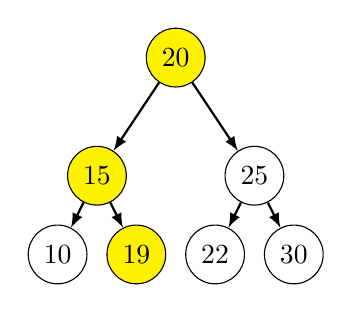
\begin{tikzpicture}[xscale=1,yscale=1]
% Styles (MODIFIABLES)
\tikzstyle{fleche}=[->,>=latex,thick]
\tikzstyle{noeud}=[fill=white,circle,draw]
\tikzstyle{feuille}=[fill=white,circle,draw]
\tikzstyle{select}=[fill=yellow,circle,draw]
% Dimensions (MODIFIABLES)
\def\DistanceInterNiveaux{1}
\def\DistanceInterFeuilles{1}
% Dimensions calculées (NON MODIFIABLES)
\def\NiveauA{(-0)*\DistanceInterNiveaux}
\def\NiveauB{(-1.5)*\DistanceInterNiveaux}
\def\NiveauC{(-2.5)*\DistanceInterNiveaux}
\def\InterFeuilles{(1)*\DistanceInterFeuilles}
% Noeuds (MODIFIABLES : Styles et Coefficients d'InterFeuilles)
\node[select] (R) at ({(1.5)*\InterFeuilles},{\NiveauA}) {$20$};
\node[select] (Ra) at ({(0.5)*\InterFeuilles},{\NiveauB}) {$15$};
\node[feuille] (Raa) at ({(0)*\InterFeuilles},{\NiveauC}) {$10$};
\node[select] (Rab) at ({(1)*\InterFeuilles},{\NiveauC}) {$19$};
\node[noeud] (Rb) at ({(2.5)*\InterFeuilles},{\NiveauB}) {$25$};
\node[feuille] (Rba) at ({(2)*\InterFeuilles},{\NiveauC}) {$22$};
\node[feuille] (Rbb) at ({(3)*\InterFeuilles},{\NiveauC}) {$30$};
% Arcs (MODIFIABLES : Styles)
\draw[fleche] (R)--(Ra);
\draw[fleche] (Ra)--(Raa);
\draw[fleche] (Ra)--(Rab);
\draw[fleche] (R)--(Rb);
\draw[fleche] (Rb)--(Rba);
\draw[fleche] (Rb)--(Rbb);
\end{tikzpicture}
\end{center}
%:-+-+-+-+- Fin

In het voorbeeld is het zoekpad naar de knoop met waarde 19 weergegeven. Dit zoekpad heeft precies complexiteit O($n$), namelijk drie stappen/vergelijkingen voordat de gezochte knoop wordt bereikt, dat is dus gelijk aan de hoogte van de boom. 
\begin{itemize}
\item Het zoekdomein bestaat aanvankelijk uit $2^n-1 = 7$ knopen, want de voorbeeldboom is een \emph{volle binaire boom}
\item Aan het begin van de zoekopdracht is er alleen een pointer naar de wortel (20). We weten dat 19 kleiner is dan de wortel, dus bezoeken we zijn linkerkind. Van de complete rechtersubboom is dus van te voren bekend dat deze niet doorzocht hoeft te worden.
\item Het zoekdomein wordt dus ineens van 7 naar $2^n-1-(2^{n-1}-1)=4$ verkleind. Voor een grote boom zijn dat veel knopen die nooit bezocht hoeven te worden.
\item De nieuwe knoop heeft waarde 15. We hebben dus nog geen resultaat, maar er is nu wel bekend dat alleen de rechtersubboom van 15 hoeft te worden doorzocht
\item Het zoekdomein is nu precies $n$ geworden, de ``worst case'' bij de binair zoeken.
\item Het rechterkind van 15 is vervolgens 19, de knoop is gevonden.
\end{itemize}
Binaire bomen zijn dus sneller dan gewone bomen tijdens het zoeken en correct mits de binaire-zoekboom-eigenschap wordt gehandhaafd. Tijdens een insert operatie kost dat inprinciepe geen extra rekenkracht, maar bij bijvoorbeeld het verwijderen moet de boom soms worden verschoven om de eigenschap te herstellen. \\
Een ander probleem is dat de binaire zoekboom eigenlijk alleen optimaal presteert als de hoogte zo gering mogelijk is voor het aantal knopen. De hoogte bepaalt namelijk de zoekcomplexiteit, niet het aantal knopen. Een binaire zoekboom met een goede balans tussen de hoogten van de subbomen is \emph{geballanceerd}. Als er tijdens het toevoegen niets bijzonders wordt gedaan, kan een binaire zoekboom heel snel ongebalanceerd raken, afhankelijk van de volgorde waarin knopen worden toegevoegd. Neem bijvoorbeeld de bovenstaande boom. Als men de knopen in de volgorde 10, 15, 19, 20, 25, 22, 30 toegevoegd ontstaat er \'e\'en lange tak naar rechts. De worst-case zoekdiepte is nu van 3 naar 7 gegaan.

%:-+-+-+- Engendré par : http://math.et.info.free.fr/TikZ/Arbre/
\begin{center}
% Racine en Haut, développement vers le bas
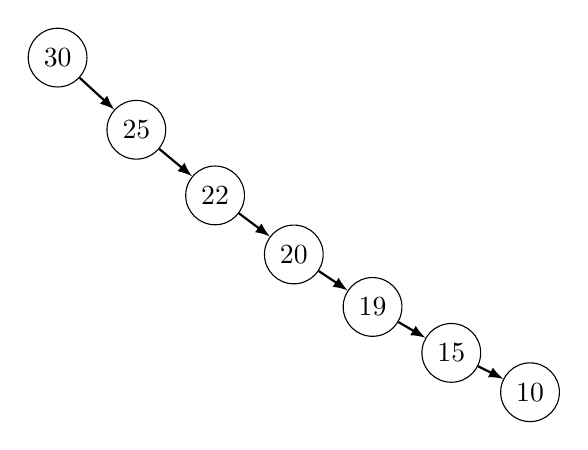
\begin{tikzpicture}[xscale=1,yscale=1]
% Styles (MODIFIABLES)
\tikzstyle{fleche}=[->,>=latex,thick]
\tikzstyle{noeud}=[fill=white,circle,draw]
\tikzstyle{feuille}=[fill=white,circle,draw]
% Dimensions (MODIFIABLES)
\def\DistanceInterNiveaux{0.5}
\def\DistanceInterFeuilles{2}
% Dimensions calculées (NON MODIFIABLES)
\def\NiveauA{(-0)*\DistanceInterNiveaux}
\def\NiveauB{(-1.8333333333333333)*\DistanceInterNiveaux}
\def\NiveauC{(-3.5)*\DistanceInterNiveaux}
\def\NiveauD{(-5)*\DistanceInterNiveaux}
\def\NiveauE{(-6.333333333333333)*\DistanceInterNiveaux}
\def\NiveauF{(-7.5)*\DistanceInterNiveaux}
\def\NiveauG{(-8.5)*\DistanceInterNiveaux}
\def\InterFeuilles{(1)*\DistanceInterFeuilles}
% Noeuds (MODIFIABLES : Styles et Coefficients d'InterFeuilles)
\node[noeud] (R) at ({(0)*\InterFeuilles},{\NiveauA}) {$30$};
\node[noeud] (Ra) at ({(0.5)*\InterFeuilles},{\NiveauB}) {$25$};
\node[noeud] (Raa) at ({(1)*\InterFeuilles},{\NiveauC}) {$22$};
\node[noeud] (Raaa) at ({(1.5)*\InterFeuilles},{\NiveauD}) {$20$};
\node[noeud] (Raaaa) at ({(2)*\InterFeuilles},{\NiveauE}) {$19$};
\node[noeud] (Raaaaa) at ({(2.5)*\InterFeuilles},{\NiveauF}) {$15$};
\node[feuille] (Raaaaaa) at ({(3)*\InterFeuilles},{\NiveauG}) {$10$};
% Arcs (MODIFIABLES : Styles)
\draw[fleche] (R)--(Ra);
\draw[fleche] (Ra)--(Raa);
\draw[fleche] (Raa)--(Raaa);
\draw[fleche] (Raaa)--(Raaaa);
\draw[fleche] (Raaaa)--(Raaaaa);
\draw[fleche] (Raaaaa)--(Raaaaaa);
\end{tikzpicture}
\end{center}
%:-+-+-+-+- Fin

De \emph{zelf-organiserende boom} is een speciaal soort binaire zoekboom die tijdens verschillende operaties probeert om de boom zo
goed mogelijk te (her)belanceren. Uiteraard kosten deze extra operaties ook meer rekenkracht en of dit zich terugbetaald in zoeksnelheid is \'e\'en van de dingen die wij zullen onderzoeken tijdens deze experimenten.

\subsection{Implementatie AVL-bomen}
Knopen van een AVL-boom hebben een \emph{balansfactor}, die altijd -1, 0 of 1 moet zijn. 
In deze implementatie is de balansfactor de hoogte van de rechtersubboom min de hoogte van de linkersubboom. 
Dit houdt dus in dat de hoogte van de linkersubboom van de wortel met maar 1 knoop kan verschillen van de hoogte van de rechtersubboom van de wortel. 
Het moment dat de balansfactor van een knoop minder dan -1 of meer dan 1 wordt, moet de boom geherstructureerd worden, om deze eigenschap te herstellen. \\

Om de balansfactor voor elke knoop te berekenen, houdt elke knoop zijn eigen hoogte bij. De balansfactor van een knoop wordt hersteld door rotaties. De richting en de hoeveelheid van de rotaties hangt af van de vorm van de betreffende (sub)boom. De volgende twee vormen en hun spiegelbeelden kunnen voorkomen bij het verwijderen of toevoegen van een knoop: \\

\begin{center}
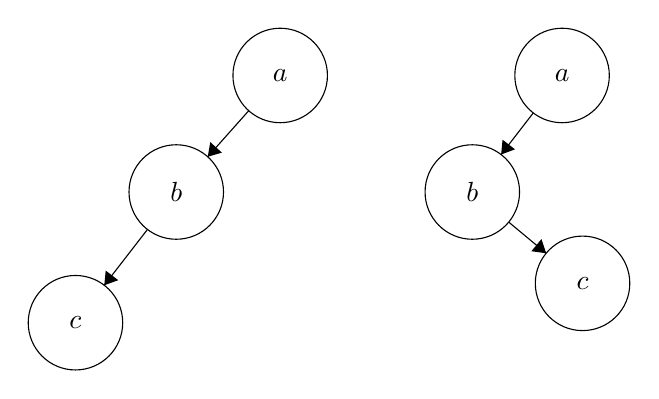
\begin{tikzpicture}[scale=0.2]
\tikzstyle{every node}+=[inner sep=0pt]
\draw [black] (16.5,-14.5) circle (3);
\draw (16.5,-14.5) node {$a$};
\draw [black] (9.9,-21.9) circle (3);
\draw (9.9,-21.9) node {$b$};
\draw [black] (34.4,-14.5) circle (3);
\draw (34.4,-14.5) node {$a$};
\draw [black] (3.5,-30.2) circle (3);
\draw (3.5,-30.2) node {$c$};
\draw [black] (28.7,-21.9) circle (3);
\draw (28.7,-21.9) node {$b$};
\draw [black] (35.7,-27.7) circle (3);
\draw (35.7,-27.7) node {$c$};
\draw [black] (14.5,-16.74) -- (11.9,-19.66);
\fill [black] (11.9,-19.66) -- (12.8,-19.4) -- (12.06,-18.73);
\draw [black] (32.57,-16.88) -- (30.53,-19.52);
\fill [black] (30.53,-19.52) -- (31.41,-19.19) -- (30.62,-18.58);
\draw [black] (31.01,-23.81) -- (33.39,-25.79);
\fill [black] (33.39,-25.79) -- (33.09,-24.89) -- (32.45,-25.66);
\draw [black] (8.07,-24.28) -- (5.33,-27.82);
\fill [black] (5.33,-27.82) -- (6.22,-27.5) -- (5.42,-26.89);
\end{tikzpicture}
\end{center}

In het eerste geval moet de wortel naar rechts worden geroteerd. In het tweede geval moeten we eerst naar de staat van de eerste subboom komen, door b naar links te roteren. Voor de spiegelbeelden van deze twee vormen geldt hetzelfde alleen in spiegelbeeld. \\

In deze implementatie van een AVL-boom bedraagt het toevoegen van een knoop in het ergste geval O($logn$) tijd, waarbij \emph{n} staat voor de hoogte van de boom. Eerst moet er gekeken worden of de data niet al in de boom voorkomt (O($logn$)) en vervolgens moet de boom op basis van de toevoeging geherstructureerd worden. Dit laatste is in het ergste geval O($logn$), omdat dan de gehele boom tot de wortel moeten worden nagelopen. \\

De complexiteitsgraad van het verwijderen van een knoop is gelijk aan die van het toevoegen van een knoop. In deze implementatie zoeken we in de rechtersubboom het kleinste kind en vervangen we de te verwijderen knoop met deze knoop. Dit heeft een duur van O($logn$). Als hij geen rechtersubboom heeft, wordt de node weggegooid en wordt zijn linkersubboom de nieuwe boom.
\subsection{Implementatie Splay-bomen}

De Splay-boom is een simpele binaire zoekboom die zichzelf herorganiseerd na elke operatie, ook na operaties die alleen lezen, zoals \texttt{find()}. Deze herorganisatiestap heet ``splay'' (vandaar de naam) en heeft ten doel de laatst aangesproken knoop bovenaan te zetten. Dit wordt dus de wortel. Hieronder is het gedrag kort samengevat:
\begin{itemize}
\item Bij zoeken wordt de gevonden knoop de wortel, mits er een zoekresultaat is.
\item Bij toevoegen wordt de toegevoegde knoop de wortel
\item Bij vervangen wordt de vervangen knoop de wortel
\item Bij verwijderen wordt de te verwijderen knoop eerst de wortel, dan wordt deze verwijderd.
\end{itemize}
Het idee achter dit gedrag is, dat vaak gebruikte knopen hoger in de boom terechtkomen en daarom sneller toegankelijk zijn voor volgende operaties. De splay-operatie zorgt er bovendien voor dat knoop die dicht in de buurt van de \emph{gesplayde} knoop zitten, ook hoger in
de boom worden geplaatst. Dit effect ontstaat doordat \emph{splay} eigenlijk een serie boom rotaties is. Als men deze rotaties
consequent uitvoerd blijft bovendien de binairy-zoekboom-eigenschap behouden.

\subsubsection{Splay}

De splay-operatie bestaat uit drie operaties en hun spiegelbeelden. We gaan uit van een knoop $n$, zijn ouderknoop $p$ en diens ouderknoop $g$. Welke operatie wordt uitgevoerd is afhankelijk van het feit of $n$ en $p$ linker- of rechterkind zijn. We definieren:
\begin{itemize}
\item De \emph{Zig} stap. Als $n$ linkerkind is van $p$ en $p$ de wortel is, doen we een rotate-right op $p$.
\item Het spiegelbeeld van \emph{Zig} is \emph{Zag}.
\item De \emph{Zig-Zig} stap. Als $n$ linkerkind is van $p$ en $p$ linkerkind is van $g$, doen we eerst een rotate-right op $g$ en dan een rotate-right op $p$.
\item Het spiegelbeeld van \emph{Zig-Zig} is \emph{Zag-Zag}
\item De \emph{Zig-Zag} stap. Als $n$ rechterkind is van $p$ en $p$ linkerkind is van $g$, doen we eerst een rotate-left op $p$ en dan een rotate-right op $g$.
\item De omgekeerde versie heet \emph{Zag-Zig}
\end{itemize}
Onze implementatie splayt op \texttt{insert(), replace(), remove()} en \texttt{find()}. De gebruiker kan eventueel zelf de splay-operatie aanroepen na andere operaties dmv de functie \texttt{splay()}.

\subsection{Implementatie Treaps}
Treap lijkt in veel opzichten op een AVL-boom. De balansfactor per knoop heeft echter plaats gemaakt voor een prioriteit per knoop. Deze prioriteit wordt bij het toevoegen van een knoop willekeurig bepaald. De complexiteit voor het toevoegen en verwijderen van een knoop is hetzelfde als bij de AVL-boom. \\

Bij het toevoegen van een knoop moet er nog steeds omhoog gelopen worden in de boom, totdat de prioriteit van de toegevoegde knoop kleiner is dan de prioriteit van de ouder. Als dit niet het geval is, blijft de toegevoegde knoop omhoog roteren. In het ergste geval kan het dus weer zo zijn dat we tot de wortel door moeten blijven lopen. \\

Bij het verwijderen van een knoop blijven we de betreffende knoop roteren naar het kind met de grootste prioriteit. Uiteindelijk belanden we dan in de situatie dat de knoop maar een of geen kinderen heeft.
In het eerste geval verwijderen we de knoop en plakken zijn subboom terug aan de boom op zijn plek en in het tweede geval verwijderen we de knoop. In het slechtste geval duurt dit dus ook O($logn$) tijd.
\section{Onderzoek}

Een praktisch voorbeeld van binair zoeken in een grote boom is de spellingscontrole. Een spellingscontrole moet zeer snel voor een groot aantal strings kunnen bepalen of deze wel of niet tot de taal behoren. Aangezien er honderduizenden woorden in een taal zitten, is
lineair zoeken geen optie. Voor onze experimenten hebben wij dit als uitgangspunt genomen en hieronder zullen we kort de experimenten toelichten die wij hebben uitgevoerd. In het volgende hoofdstuk staan vervolgens de resultaten beschreven.

\subsection{Hooiberg}

``Hooiberg'' is de naam van het testprogramma dat we hebben geschreven speciaal ten behoeven van onze experimenten.
Het is een klein console programma dat woorden uit een bestand omzet tot een boom in het geheugen. 
Deze boom kan vervolgens worden doorzocht met de input uit een ander bestand: de ``naalden''.
De syntax is alsvolgt:
\begin{verbatim}
hooiberg type hooiberg.txt naalden.txt [treap-random-range]
\end{verbatim}
Hierbij is \texttt{type} \'e\'en van \texttt{bst, avl, splay, treap}, het eerste bestand bevat de invoer voor de boom, het tweede bestand een verzameling strings als zoekopdracht en de vierde parameters is voorbehouden voor het type \texttt{treap}.
De bestanden kunnen woorden of zinnen bevatten, gescheiden door regeleinden. De binaire bomen gebruiken lexicografische sortering 
die wordt geleverd door de operatoren \texttt{<} en \texttt{>} van de klasse \texttt{std::string}. Tijdens het zoeken wordt een
exacte match gebruikt (case-sensitive, non-locale-aware).

\subsection{Onderzoeks(deel)vragen}

Met onze experimenten hebben we gepoogd een aantal eenvoudige vragen te beantwoorden over het gebruik van de verschillende
binaire en zelf-organiserende bomen, te weten:

\begin{itemize}
\item Hoeveel meer rekenkracht kost het om grote datasets in te voegen in zelf-organiserende bomen tov binaire bomen?
\item Levert een zelf-organiserende boom betere zoekprestaties en onder welke opstandigheden?
\item Hoeveel extra geheugen kost een SOT?
\item Wat is de invloed van de random-factor bij de Treap?
\end{itemize}

\subsection{Meetmethoden}

Om de bovenstaande vragen te toetsen, hebben we een aantal meetmethoden bedacht.

\begin{itemize}
\item Rekenkracht hebben we gemeten in milliseconden tussen aanvang en termineren van een berekening. We hebben de delta's berekend rond de relevante code blokken dmv de C++11 \texttt{chrono} klassen in de Standard Template Library. Alle test zijn volledig sequentieel en single-threaded uitgevoerd. Deze resultaten zijn representatie voor \'e\'en bepaald systeem, vandaar dat we aantal \% `meer rekenkracht' als eenheid gebruiken.
\item Zoekprestatie hebben we zowel met rekenkracht als zoekdiepte gemeten. De zoekdiepte is het aantal stappen dat vanaf de wortel moet worden gemaakt om bij de gewenste knoop te komen. We hebben hierbij naar het totaal aantal stappen gekeken en naar de gemiddelde zoekdiepte.
\item Geheugen hebben we gemeten met de \texttt{valgrind} memory profiler. Dit programma wordt gebruikt voor het opsporen van geheugen lekken en houdt het aantal allocaties op de heap bij. Dit is representatie voor het aantal gealloceerde nodes. Aangezien hooiberg nauwelijks een eigen geheugen-voetafdruk heeft, zijn deze waarden representatief.
\end{itemize}

\subsection{Input data}

Voor ons experiment hebben we een taalbestand gebruikt van OpenTaal.org met meer dan 164.000 woorden. Dit is een relatief klein taalbestand, maar voldoede om verschillen te kunnen zien. We hebben een aantal testcondities gebruikt:
\begin{itemize}
\item Voor het inladen een wel of niet alfabetisch gesoorteerd taalbestand gebruiken.
\item Als zoekdocument hebben we een gedicht met 62 woorden gebruikt. Er zitten een aantal dubbele woorden in alsook een aantal woorden die niet in de woordenlijst voorkomen (werkwoordsvervoegingen).
\item We hebben \'e\'en conditie waarbij we de random-range van de Treap hebben gevari\"eerd.
\end{itemize}

\subsection{Hypothesen}

\begin{itemize}
\item De binairy search tree zal vermoedelijk het snelst nieuwe data toevoegen. De splay tree heeft veel ingewikkelde rotatie bij een insert, dus deze zal het traagst zijn.
\item Bij het gedicht zal de splay boom waarschijnlijk het snelst zijn omdat deze optimaliseert voor herhalingen.
\item De bomen die een aparte node-klasse gebruiken (avl en treap) gebruiken het meeste geheugen.
\item De meest effici\"ente randomfactor is afhankelijk van de grootte van de boom die geïmplementeerd gaat worden. Bij een kleine boom volstaat een kleine randomfactor, bij een grote boom volstaat een grote randomfactor.
\end{itemize}

\section{Resultaten}
Voor elke soort boom hebben we elk experiment tien keer uitgevoerd.

\subsection{Experiment 1}
\subsubsection{Deelexperiment 1}
In dit experiment hebben we voor elke soort boom gemeten hoe lang het duurt de boom op te bouwen met het bestand  \texttt{Nederlands\_unsorted.txt} om deze tijden te kunnen vergelijken. Dit hebben we gemeten in miliseconden. De volgende gegevens kwamen eruit. Deze hebben we vervolgens verwerkt in een grafiek. \\

\resizebox{\linewidth}{!}{
\begin{tabular}{c c c c c c c c c}
 & BST & Treap(10) & Treap(100) & Treap(1000) & Treap(10000) & Treap(100000) & AVL & Splay \\
 & 525 & 1160 & 1526 & 1307 & 1272 & 1368 & 1063 & 1065 \\
 & 527 & 1162 & 1409 & 1332 & 1202 & 1736 & 1207 & 1059 \\
 & 511 & 1173 & 1215 & 1181 & 1846 & 1669 & 1102 & 1053 \\
 & 585 & 1141 & 1298 & 1547 &  	1246 & 1688 & 1150 & 1202 \\
 & 589 & 1319 & 1427 & 1190 & 1538 & 1221 & 1146 & 1067 \\
 & 588 & 1265 & 1560 & 1472 & 1271 & 1238 & 1251 & 1063 \\
 & 592 & 1464 & 1428 & 1338 & 1286 & 1543 & 1136 & 1050 \\
 & 492 & 1501 & 1704 & 2594 & 1316 & 1206 & 1155 & 1092 \\
 & 506 & 1425 & 1449 & 1269 & 1571 & 1389 & 1153 & 1183 \\
 & 512 & 1391 & 1474 & 1384 & 1440 & 1663 & 1203 & 1162 \\
GEM & 542,7 & 1300,1 & 1449 & 1461,4 & 1398,8 & 1472,1 & 1156,6 & 1099,6 
\end{tabular}
}

\begin{center}
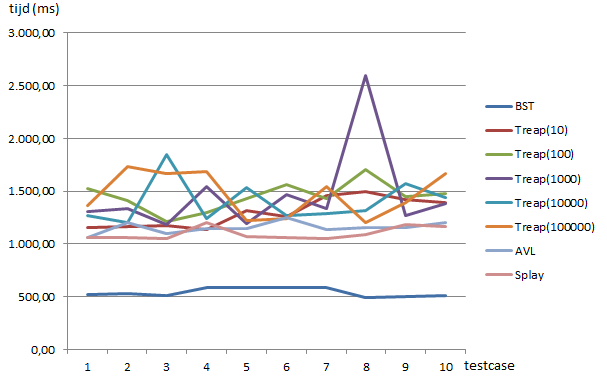
\includegraphics[scale=0.75]{fill.png}
figuur 1. Grafiek over het aantal ms voor het construeren van een graaf.
\end{center}

\subsubsection{Deelexperiment 2}
Het vullen van de boom met de alfabetische woordenlijst levert, zoals eerder beschreven, een diagonale lijn van data in de binaire zoekboom op, waar we niet efficiënt in kunnen zoeken. Treap doet het ook niet veel beter in dit gebied, waar de gemiddelde zoektijd met \texttt{gedicht.txt} bij binaire zoekbomen rond de 167,5 miliseconden ligt, ligt hij bij treap rond de 253,5 miliseconden. De gemiddelde zoektijd voor zowel AVL-bomen als splaybomen is echter nooit meer dan 1 miliseconde. \\
Dit verschil is overigens ook opvallend bij het vullen van de boom, waar splay en AVL gelijk presteren als in experiment 1, duurt het bij zowel de binaire zoekboom als de treap bijna een factor van 100 langer.

\subsection{Experiment 2}
\subsubsection{Deelexperiment 1}
Om de zoekprestaties van de verschillende soorten bomen te vergelijken kijken we naar zowel de totale zoekdiepte van de boom, de gemiddelde zoekdiepte van een woord in \texttt{gedicht.txt} en naar het aantal miliseconden die de gemiddelde zoekoperatie nodig had. Onze boom is opgebouwd uit \texttt{nederlands\_unsorted.txt}.
De gehele hoogte van de boom die dit opleverd en de gemiddelde zoekdiepte van een woord uit \texttt{gedicht.txt} staan in onderstaande tabel weergegeven. Het gemiddelde aantal miliseconden dat nodig was voor de zoekoperaties van elk woord bedroeg nooit meer dan 1 miliseconden en dook zelfs vaak onder de halve miliseconde.

\begin{center}
\begin{tabular}{c c c}
Type & totale zoekdiepte & gemiddelde zoekdiepte \\
Treap(10) & 1843,5 & 32,5 \\
Treap(100) & 2256,9 & 39,9 \\
Treap(1000) & 2275,2 & 40,2 \\
Treap(10000) & 2268,7 & 39,9 \\
Treap(100000) & 2205,8 & 39 \\
BST & 1106 & 19 \\
AVL & 880 & 15 \\
splay & 997 & 17 \\
\end{tabular}
\end{center}

\subsubsection{Deelexperiment 2}
Ditzelfde experiment voerden we uit op dezelfde boom met als zoekopdrachten elk element in die boom. Daar kwamen de volgende resultaten uit. \\

\begin{center}
\begin{tabular}{c c c c}
Type & totale zoekdiepte & gemiddelde zoekdiepte & tijd (ms) \\
Treap(10) & 5783309 & 34,67 & 882.005 \\
Treap(100) & 7034043 & 42,22 & 956.880 \\
Treap(1000) & 7162473 & 44.11 & 1067.861 \\
Treap(10000) & 7253419 & 44,67 & 1053.257 \\
BST & 3369405 & 20 & 557.934 \\
AVL & 2576171 & 15 & 450.390 \\
splay & 3922834 & 23 & 1378,197  \\
\end{tabular}
\end{center}

\subsection{Experiment 3}
Hieronder staan de hoeveelheden geheugen en het aantal allocaties weergegeven voor elke boom. De metingen zijn van heap dynamisch gealloceerd geheugen alleen en zijn uitgevoerd met Valgrind. \\
\begin{center}
\begin{tabular}{c c c}
Type & allocs & bytes \\
Treap & 493280 & 16704426 (15,9 Mb) \\
BST & 493278 & 15389858 (14,7 Mb) \\
AVL & 493279 & 16704390 (15,9 Mb)\\
splay & 493260 & 15389922 (14,7 Mb)\\
\end{tabular}
\end{center}
\subsection{Experiment 4}
\subsubsection{Deelexperiment 1}
Bij dit experiment zijn we gaan zoeken naar de sleutelwoorden van \texttt{gedicht.txt} in \texttt{Nederlands\_unsorted.txt}. De resultaten hiervan staan in onderstaande tabelen weergegeven, waarbij de eerste rij staat voor de mate van willekeurigheid van de prioriteit (hoe hoger, hoe willekeuriger). \\

Gemiddelde zoekdiepte voor zoekopdrachten \\
\begin{center}
\begin{tabular}{c c c c c c}
 & 10 & 100 & 1000 & 10000 & 10000 \\
 & 34 & 36 & 36 & 45 & 38 \\
 & 31 & 40 & 49 & 34 & 47 \\
 & 29 & 	35 & 26 & 70 & 41 \\
 & 32 & 	40 & 35 & 41 & 42 \\
 & 33 & 	44 & 32 & 38 & 36 \\
 & 34 & 	40 & 49 & 33 & 37 \\
 & 35 & 	47 & 29 & 37 & 35 \\
 & 36 & 	47 & 66 & 36 & 29 \\
 & 32 & 	34 & 36 & 35 & 39 \\
 & 29 & 	36 & 44 & 30 & 46 \\
GEM & 32,5 & 39,9 & 40,2 & 39,9 & 39 \\
\end{tabular}
\end{center}

Totale zoekdiepte\\
\begin{center}
\begin{tabular}{c c c c c c}
 & 10 & 100 & 1000 & 10000 & 10000 \\
 & 1914 & 2041 & 2017 & 2549 & 2173 \\
 & 1745 & 2254 & 2752 & 1957 & 2657 \\
 & 1652 & 1982 & 1511 & 3954 & 2312 \\
 & 1836 & 2261 & 1983 & 2310 & 2366 \\
 & 1861 & 2482 & 1819 & 2169 & 2033 \\
 & 1925 & 2253 & 2783 & 1852 & 2092 \\
 & 2002 & 2656 & 1643 & 2126 & 1947 \\
 & 2032 & 2672 & 3732 & 2059 & 1658 \\
 & 1798 & 1917 & 2021 & 1999 & 2211 \\
 & 1670 & 2051 & 2491 & 1712 & 2609 \\
GEM & 1843,5 & 2256,9 & 2275,2 & 2268,7 & 2205,8 \\
\end{tabular}
\end{center}

\subsubsection{Deelexperiment 2}
De volgende tabel geeft de uitersten aan van de resultaten die we tegenkwamen in deelexperiment 2 van experiment 2. \\

\begin{center}
\begin{tabular}{c c c c c c c}
 & \multicolumn{2}{c}{Totale zoekdiepte} & \multicolumn{2}{c}{Gemiddelde zoekdiepte} & \multicolumn{2}{c}{Tijd}\\ 
bereik & minimum & maximum & minimum & maximum & minimum & maximum \\
10 & 5194145 & 6826579 & 31 &  41 & 778.449 & 992.709 \\
100 & 5321940 & 10137343 & 32 & 61 & 823.003 & 1379.380 \\
1000 & 592787 2& 9952377 & 32 & 60 & 873.975 & 1300.820 \\
10000 & 5841811 & 10283676 & 35 & 62 & 940.451 & 1270.090 \\
\end{tabular}
\end{center}
\section{Conclusies}
\begin{itemize}
\item Het vullen van een niet-zelf-balanceerdende binaire zoekboom met een niet-gesorteerde verzameling is meer dan twee keer zo effici\"ent als het vullen van een variant die wel zelf-balancerend is. Dat is eigenlijk ook wat men mag verwachten gezien het feit dat de zelf-balancerende bomen met operaties moeten uitvoeren om de balans te herstellen.
\item De binaire zoekboom en de treap laten presteren erg slecht zodra we een boom moeten vullen met een gesorteerde verzameling. Dit is zichtbaar in de resultaten van experiment 1. Zie ook de uitgebreide uitleg hierover in sectie 2, \emph{Implementatie Binaire zoekboom}.
\item Een AVL-boom voert een zoekopdracht gemiddeld het snelste uit. Dit is anders dan voorspelt bij onze hypothese dat de splay boom sneller zou moeten presteren bij zoekacties met herhalende patronen. Dit zou mogelijk veroorzaakt kunnen worden door het feit dat van alle bomen de AVL-boom het beste gebalanceerd blijft, omdat hier de prioriteit ligt van het algoritme. Het algoritme achter de splay-boom prioriteert juist op meest recente toegang, maar niet per se op de balans in de boom vanaf de wortel. 
\item Treaps en AVL-bomen nemen het meeste geheugen in het gebruik. Zie experiment 3. Dit is in overeenstemming met onze hypothese.
\item De onderlinge verschillen wat betreft geheugenverbruik zijn, zelfs met een wat grotere data set, verwaarloosbaar. Niet geheel verassend nemen de nodes van Treap en AVL iets meer ruimte in omdat deze een prioriteit resp. balansfactor bijhouden.\\
Het feit dat het invoerbestand \texttt{Nederlands\_unsorted.txt} slechts 2,1 Mb groot is, zegt wel iets over de effici\"entie van het geheugengebruik in het algemeen, zowel van onze implementatie als van dit soort boom datatypen in het algemeen.
\item Ontwerpkeuzen spelen bij bovenstaande een grote rol: als we bijvoorbeeld ervoor hadden gekozen om geen 'ouder-pointers' te gebruiken, hadden we tussen 0,6 en 1,2 Mb op deze cijfers kunnen besparen. 
\item Des te minder willekeurig de prioriteit van een Treap, des te effici\"enter het uitvoeren van een zoekopdracht.
\item Treap presteert niet consistent, dit blijkt uit deelexperiment 2 van experiment 4. Dit is vooral merkbaar bij een prioriteit met een grote mate van willekeurigheid, waar in het experiment de best-case testcase een minimum gemiddelde zoekdiepte van 35 heeft en de worst-case testcase een maximum gemiddelde zoekdiepte van 62 heeft.
\end{itemize}
\section{Appendix}

\subsection{hooiberg.cc}
\lstinputlisting{../src/hooiberg.cc}
\subsection{Tree.h}
\lstinputlisting{../src/Tree.h}
\subsection{TreeNode.h}
\lstinputlisting{../src/TreeNode.h}
\subsection{TreeNodeIterator.h}
\lstinputlisting{../src/TreeNodeIterator.h}
\subsection{SelfOrganizingTree.h}
\lstinputlisting{../src/SelfOrganizingTree.h}
\subsection{BinarySearchTree.h}
\lstinputlisting{../src/BinarySearchTree.h}
\subsection{BSTNode.h}
\lstinputlisting{../src/BSTNode.h}
\subsection{AVLTree.h}
\lstinputlisting{../src/AVLTree.h}
\subsection{AVLNode.h}
\lstinputlisting{../src/AVLNode.h}
\subsection{SplayTree.h}
\lstinputlisting{../src/SplayTree.h}
\subsection{Treap.h}
\lstinputlisting{../src/Treap.h}
\subsection{TreapNode.h}
\lstinputlisting{../src/TreapNode.h}
\end{document}